% When Does Prefix-Aware Routing Pay? -- preprint draft.
% Every number here comes from a committed results file; paper/README.md maps each table and figure
% to its source. Build: `tectonic main.tex` (or pdflatex on Overleaf/arXiv). ASCII-only on purpose,
% so pdfLaTeX (arXiv's default) and XeTeX both compile it.
\documentclass[10pt,twocolumn]{article}
\usepackage[letterpaper,margin=0.75in,columnsep=0.25in]{geometry}
\usepackage[T1]{fontenc}
\usepackage{newtxtext,newtxmath}
\usepackage{microtype}
\usepackage{booktabs}
\usepackage{graphicx}
\usepackage{xcolor}
\usepackage[font=small,labelfont=bf,skip=4pt]{caption}
\usepackage{enumitem}
\usepackage[hidelinks]{hyperref}
\setlist{nosep,leftmargin=*}

\newcommand{\todo}[1]{\textcolor{red}{[TODO: #1]}}
\newcommand{\PA}{\textsc{pa}}
\newcommand{\SSt}{\textsc{ss}}
\newcommand{\RR}{\textsc{rr}}
\newcommand{\LL}{\textsc{ll}}
\newcommand{\miss}{--}

\title{When Does Prefix-Aware Routing Pay?\\[3pt]
\large A vLLM-Calibrated, Pre-Registered Study of KV-Cache Routing Across Replicas}
\author{Harshit\thanks{Independent researcher. \todo{affiliation and e-mail}. Code, configurations,
results and the dated registration log: \url{https://github.com/TODO/kv-routing-sim}.}}
\date{Draft of \today}

\begin{document}
\maketitle

\begin{abstract}
Serving a large language model on several replicas forces a routing decision for every request, and
that decision sets how much of each replica's prefix (KV) cache is reused. We ask when sending a
request to the replica that already caches its prefix beats keeping each user's session on one
replica, and what the choice costs in GPUs. We build a trace-driven multi-replica simulator whose
cache model follows vLLM~0.30.0's block pool, and check it against a live engine before using it:
with predictions committed in advance, it reproduces every prefix-cache counter exactly on two
sequential workloads under eviction pressure, and predicts the hit rate within 0.3\% on a concurrent
one, where a plain LRU model is off by 19.7\%. On two live replicas under the traffic of our finding
it predicts every hit rate within 1.4\% and the order of the policies; its timing model, however,
under-predicts latency there by 5--222$\times$, so the replica counts below are simulator figures and
optimistic. With timings fitted on a Tesla~T4 and each hypothesis registered before it ran, we find
that one ratio decides the policy: the working set of the tenants' system prompts over one replica's
cache. With one shared prompt (0.06 of a cache), session-sticky routing holds a 2\,s p95
time-to-first-token on 2~simulated T4s where round-robin needs~3. With 64 prompts
(2.66 caches), prefix-affinity with a load weight holds it on~5 (4 with a smaller weight, found
after the test) and session-sticky cannot hold it on~8. Prefix-affinity without a load weight
collapses whenever one prompt dominates. The direction of this flip survives four rescalings of the
hardware's speed; the replica counts and the full policy ranking do not (Kendall's $\tau_b$ as low
as 0.51). On real traces, session-sticky and prefix-affinity come within one replica of each other:
on Mooncake, whose prompts are shared across users, and on AgentX's coding-agent sessions, where
nothing is. Prefix-affinity without a load weight fails at every load on the first and matches
session-sticky on the second, so its collapse comes from shared prompts.
\end{abstract}

\section{Introduction}

Large language models are usually served by several identical replicas behind a router. Each replica
keeps a prefix cache: vLLM stores the key-value (KV) blocks of earlier prompts and reuses them when a
new prompt begins the same way~\cite{kwon2023}, and SGLang does the same with a radix
tree~\cite{zheng2023}. Agentic and multi-turn traffic repeats a great deal --- every request of a
tenant carries the same system prompt, and every turn of a session re-sends the session's history ---
so reuse can remove most of the prefill work. But a replica can reuse only what it holds. The router
therefore decides the hit rate: a request that lands where its prefix is cached skips that prefill;
the same request sent elsewhere pays for it again.

Operators choose among three families of policy. Load balancers (round-robin, least-loaded,
power-of-two choices) ignore the cache. Session affinity keeps every turn of a session on one
replica, capturing the session's own history. Prefix affinity sends a request to the replica with the
longest cached match, capturing prefixes shared across users as well, usually tempered by a load
term~\cite{srivatsa2024}; production routers such as SGLang's cache-aware router~\cite{sglang},
NVIDIA Dynamo's KV router~\cite{dynamo} and llm-d's scheduler~\cite{llmd} combine a prefix signal and
a load signal under operator-set weights or thresholds. Which family to run, and on how many GPUs, is
mostly decided by intuition, and measuring it on real fleets is expensive.

We answer the question with a simulator that we first checked against a live engine, and with
hypotheses committed to a public log before each experiment ran. Our contributions:
\begin{itemize}
\item A trace-driven multi-replica simulator whose cache model follows vLLM~0.30.0's block pool. With
  predictions committed before the run, it reproduces a live engine's prefix-cache counters exactly
  on two sequential workloads under eviction pressure, and within 0.3\% on a concurrent one; on two
  live replicas it predicts every hit rate within 1.4\%, though latency is far worse than its timing
  model predicts (\S\ref{sec:calibration}).
\item A finding from a registered test: the policy is decided by the ratio of the tenants' prompt
  working set to one replica's cache. Below it, session affinity needs the fewest replicas; above it,
  prefix affinity with a load weight does, and session affinity fails. Prefix affinity without a load
  weight collapses whenever one prompt dominates (\S\ref{sec:finding}).
\item Three tests that could have broken the finding. Rescaling the hardware's speed keeps its
  direction but not its replica counts, so replica counts must be measured on the target GPU
  (\S\ref{sec:hardware}). On two real trace families the many-prompt advantage does not appear and
  the two good policies tie within a replica; but the traces bracket the mechanism, since pure
  prefix affinity fails exactly where prompts are shared across users (\S\ref{sec:real}).
\end{itemize}
Code, configurations, raw results with their provenance, and the dated log of every registration and
outcome --- including four falsified hypotheses --- are public.

\section{Background and related work}

\paragraph{Prefix caching.} vLLM manages KV memory in fixed-size blocks and caches each full block
under a hash of its entire prefix~\cite{kwon2023}; a freed block stays reusable until the pool needs
it. Only full blocks are shared, so the block (16 tokens here) is the unit of reuse. SGLang's
RadixAttention keeps the same information in a radix tree~\cite{zheng2023}.

\paragraph{Routing and scheduling across replicas.} Preble schedules prompts across GPUs by trading
prefix locality against load~\cite{srivatsa2024}. Llumnix rebalances load across instances with live
migration~\cite{sun2024}. Mooncake builds a KV-cache-centric, disaggregated serving architecture and
released the request traces we replay~\cite{qin2024,mooncaketraces}. CacheWise pairs prefix-aware
scheduling with reuse-aware eviction for coding agents~\cite{tiwari2026}, and agentic-kv-cache
replays single-engine eviction policies on the AgentX and Mooncake traces we also use, finding LRU
hard to beat~\cite{agentickv}; both work inside one engine. Our results on the load
weight (\S\ref{sec:alpha}) bear on how routers that mix prefix and load signals set it.

\paragraph{Simulators.} Vidur established trace-driven simulation of LLM serving and uses it to
search deployment configurations~\cite{agrawal2024}. Its main branch has no prefix cache; its
\texttt{canary} branch carries a block-level prefix cache and prefix-cache-aware routers that have not
been merged. Frontier adds prefix and hierarchical caching, session-sticky routing and SLA-aware
configuration search~\cite{feng2026}; it has no prefix-affinity router,\footnote{As of September
2026.} so a system prompt shared by different users is invisible to its routing. disagg-sim
implements a radix prefix cache with a KV-aware router and reports the tension between locality and
load on synthetic workloads, without live-engine calibration~\cite{disaggsim}. We claim no new
mechanism. What this work adds is the combination: a cache model checked counter by counter against a
live engine, registered tests of when prefix affinity pays, and replica sizing with a cost, on
generated and real traces.

\section{Simulator}\label{sec:sim}

\paragraph{Traces.} A request is its arrival time, its prompt as a chain of block hashes, its prompt
and output lengths, and an optional session id. No text enters the simulator, so a production trace
can be replayed without its prompts. Adapters convert serving logs and published traces to this form.

\paragraph{Replicas.} Each replica is an event-driven model of a vLLM engine: continuous batching up
to \texttt{max\_num\_seqs} requests, a prefill step whose cost grows with the uncached prompt tokens,
and a decode step whose cost grows with the batch. Its cache follows vLLM~0.30.0's block pool, with
each behaviour tied to a line of vLLM's source: blocks leave a free queue in vLLM's order; a cached
block is evicted only when no free block remains; full blocks of generated tokens are cached as well;
a request is admitted only when its blocks fit; and when a running request cannot grow, the most
recently admitted request is preempted and later recomputed. The hit rate is computed as vLLM reports
it: prefix-cache hits over queries, in tokens. A plain LRU cache over prompt blocks is kept as an
ablation.

\paragraph{Policies.} Seven routers see the fleet state and each request: round-robin (\RR);
least-loaded (\LL, fewest outstanding requests); power-of-two choices; consistent hashing on the
prompt's first four blocks; session-sticky (\SSt: a session's first request goes to the least-loaded
replica and later turns follow it); prefix-affinity (\PA: the replica with the longest match in the
router's own map of the blocks it has dispatched, which --- like production routers --- does not see
evictions); and \PA{} with load weight $\alpha$ (\PA$_\alpha$: score $=$ matched blocks $-\ \alpha
\times$ outstanding requests). Ties are broken by a seeded random stream, and every configuration is
repeated over seeds.

\paragraph{Service level and cost.} A configuration meets the service level if its p95
time-to-first-token (TTFT) is at most 2\,s --- MLPerf's limit for conversational
serving~\cite{mlperf}, which MLPerf applies at the 99th percentile, so ours is looser. For each
policy, the required replica count $R$ is the fewest replicas from 1 to 8 that meet it on every seed.
Cost is rupees per 1{,}000 successful requests at the on-demand price of a g4dn.xlarge (one T4,
USD~0.526 per hour~\cite{awsprice}, INR~95.87 per USD~\cite{fedh10}); it matters only between policies
that tie on~$R$.

\paragraph{Protocol.} Every hypothesis, decision rule and threshold was committed to the repository
before its experiment ran: the design in a configuration file, the rules in a dated entry of a public
log. Results are appended as new entries, falsified ones included; earlier entries are never edited.
Anything chosen after seeing a result is labelled \emph{post hoc}. Each results file records the
commit, whether the working tree was clean, the seeds, the hardware and the installed package
versions.

\section{Calibration against a live engine}\label{sec:calibration}

\paragraph{Setup.} vLLM~0.30.0 (V1 engine, asynchronous scheduling on, its default) served Qwen3-4B in
fp16 on a Tesla~T4 with 16-token blocks. We fixed the cache at 512 blocks (511 usable) so that it
overflows and its capacity is an exact input. The workload was 120 agentic requests (40 sessions of 3
turns sharing one system prompt), replayed one at a time with 1-token outputs (W2) and 64-token
outputs (W1), and concurrently (W3), three runs each. The simulator's predictions were committed
before the runs.

\begin{table}[t]
\centering\small
\caption{Hit rate of a live vLLM~0.30.0 against the two cache models (Qwen3-4B, T4, a 512-block
cache). Engine: three runs per workload; the sequential runs were identical, W3 shows the mean.}
\label{tab:calib}
\begin{tabular}{@{}lccc@{}}
\toprule
Workload & Engine & Block pool & LRU \\
\midrule
W2: sequential, 1-token out  & 0.6090 & 0.6090 & 0.6073 \\
W1: sequential, 64-token out & 0.4883 & 0.4883 & 0.6073 \\
W3: concurrent               & 0.5076 & 0.509  & 0.6073 \\
\quad W3 preemptions         & 27     & 24     & 0 \\
\quad W3 p95 TTFT (s)        & 41.0   & 38.3   & 11.2 \\
\bottomrule
\end{tabular}
\end{table}

\paragraph{Result.} On both sequential workloads the block-pool model reproduces the engine exactly
(Table~\ref{tab:calib}): every counter, and every request's cached-token count, in all six runs. The
LRU ablation agrees only when requests hold no decode blocks (W2, within 0.17 points). With 64-token
outputs it over-predicts the hit rate by 11.9 points, because vLLM caches full decode blocks, which
are almost never reused but occupy the same small cache and evict useful prefixes. On the concurrent
workload, with a timing profile fitted without it, the block-pool model predicts the hit rate within
0.3\%, 24 preemptions against the engine's 27, and the p95 TTFT within 6.7\%. LRU neither makes
requests wait for memory nor preempts them, and under-predicts the p95 TTFT by 73\%. The engine's
block-eviction histograms agree in count (963 and 1{,}880 events) and, on W2, bucket for bucket.

\paragraph{Timing and capacity.} On the T4, prefill costs 0.70\,ms per uncached token ($R^2 = 0.93$)
and a decode step $52.9 + 1.23\,b$\,ms for a batch of $b$ ($R^2 = 0.58$). Two errors are known and
kept rather than tuned away: a single sequence decodes slower (63.6\,ms per token) than the line
predicts, and an idle replica's TTFT is over-estimated by about 20\,ms. In the fleet experiments each
replica has the capacity vLLM itself allocated on a T4 for this model, 1{,}537 blocks; our estimate
from memory arithmetic had been 56\% too high. An earlier check with round-robin across two physical
T4s predicted the recomputed prefill tokens exactly (1{,}088).

\paragraph{Two live replicas.} We then registered a test of the finding's mechanism on two vLLM
servers, one per physical T4, each with its natural 1{,}537 blocks: the traffic of \S\ref{sec:finding}
at 1 session per second (120 sessions of 4 turns), with one shared prompt (K1) and with 64 (K64),
routed by round-robin, session-sticky and prefix-affinity, ported from the simulator. It held only if
every run's hit rate came within 10\% of its prediction (S1) and every pair of policies predicted at
least 0.02 apart came out in the same order (S2). The notebook ran twice, and both runs held
(Table~\ref{tab:twolive}): every hit rate within 1.4\% (the K1 runs to four decimals), and all five
tested pairs in order, including prefix-affinity above session-sticky at K64. Latency was predicted
but not tested, and there the timing model failed: p95 TTFT came out 5--222$\times$ the prediction,
and four of the five runs predicted to preempt nothing preempted 15--83 times. The client sent every request on time; the
engines were overloaded. From vLLM's own statistics, decode steps took 2.7--4.0$\times$ what the
fitted profile says at every batch size, which at two requests per second per engine is enough to
start the spiral of queueing, a full cache, preemption and recomputation. The order of the policies
by p95 TTFT still matched the prediction in both workloads and both runs --- an observation, not a
test. Two causes are possible and neither is tested: the profile has no context-length term, and
these prompts are about 1{,}700 tokens; or CPU contention between two engines and a client on four
vCPUs. A packaged calibration command run on a fresh T4 engine is consistent with the first. It reproduced
that engine's counters exactly on a separate check (48 of 48 requests), and its prefill measurements
cost 0.71\,ms per token up to 1{,}024 tokens --- the value above --- but 1.12\,ms at 2{,}040, a curve no
straight line fits.

\begin{table}[t]
\centering\small
\caption{Two live T4 replicas at 1 session/s: prediction against two runs. Hit rate was the
registered test; p95 TTFT (seconds) was predicted but not tested.}
\label{tab:twolive}
\begin{tabular}{@{}lcccc@{}}
\toprule
 & \multicolumn{2}{c}{Hit rate} & \multicolumn{2}{c}{p95 TTFT (s)} \\
Run & predicted & live & predicted & live \\
\midrule
K1 round-robin     & 0.880 & 0.880 & 0.44 & 11--15 \\
K1 session-sticky  & 0.921 & 0.921 & 0.35 & 1.8--1.9 \\
K1 prefix-affinity & 0.923 & 0.923 & 0.48 & 106--107 \\
K64 round-robin    & 0.694 & 0.695 & 5.8  & 108--111 \\
K64 session-sticky & 0.821 & 0.810--0.822 & 1.55 & 57--72 \\
K64 prefix-affinity & 0.844 & 0.844--0.846 & 1.26 & 32--39 \\
\bottomrule
\end{tabular}
\end{table}

\section{Results}

Every replica count in this section is the simulator's, on the T4 profile of
\S\ref{sec:calibration}; for prompts of this length that profile proved optimistic on live engines,
so the counts are best read as relative, not absolute.

\subsection{One shared prompt: session affinity wins}\label{sec:one}

The first sweep used 200 sessions of 4 turns (a 150-token context, 40-token user and 60-token
assistant turns, 64 output tokens, 6\,s between turns) sharing one system prompt, with cross-session
sharing of 0.3 or 0.8; 1--8 sessions per second; seven policies; 1--8 replicas; five seeds. \SSt{}
needed the fewest replicas at every load on both traces --- from 2 sessions per second, 25--43\% fewer
than \RR{} --- by spreading
sessions evenly (load imbalance at most 1.09) while keeping each session's history on its replica.
\PA{} sent every new session to the replica holding the shared prompt: its load imbalance equalled
the number of replicas, it preempted 110--212 times per run and so evicted the prefix it was
protecting, and from 2 sessions per second no fleet of up to 8 held the service level.

We had registered (H2) that \PA{} would beat \LL{} below some boundary in sharing and load. The
boundary ran the other way: \PA{} beat \LL{} only when no prompt was shared at all, and once any was,
it lost at every load from 2 sessions per second, by 60--260\,s of p95 TTFT. A registered sweep of the
load weight on the first sweep's traces, $\alpha \in \{1, 2, 4, \ldots, 64\}$, gave total required
replicas over its 12 (trace, load) points of 64, 57, 58, 48, 45, 48 and 49; $\alpha^* = 16$ was then
fixed for the tests below. Even at $\alpha^*$, \PA$_\alpha$ needed more replicas than \SSt{} (45
against 36 in total).

\begin{figure*}[t]
\centering
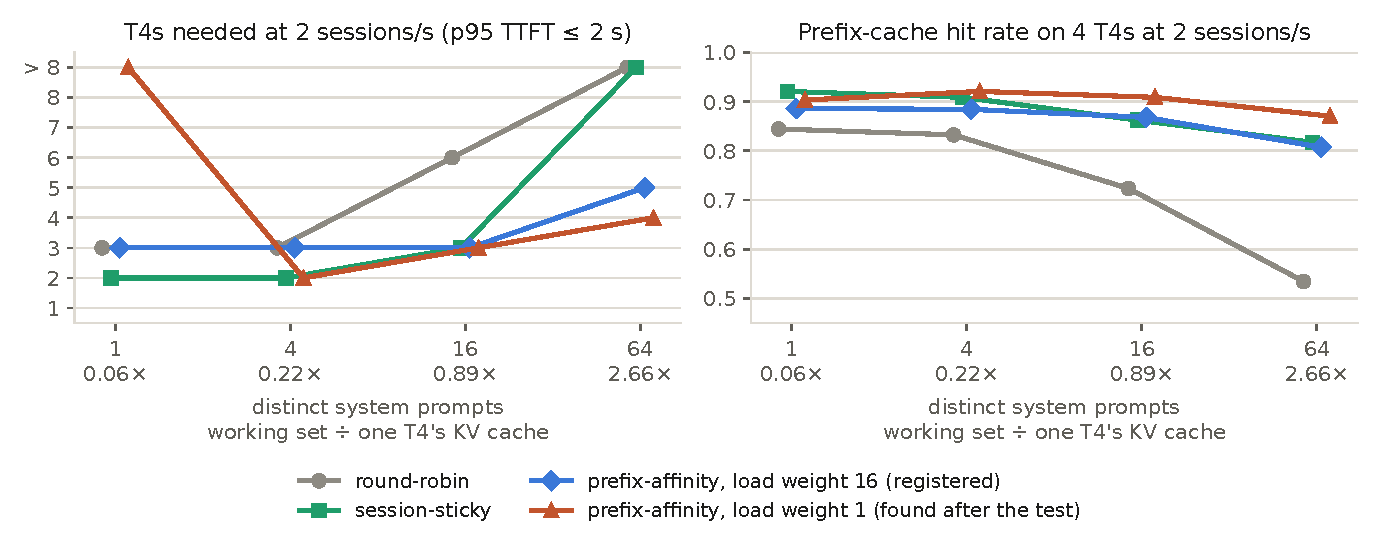
\includegraphics[width=0.94\textwidth]{figures/flip.pdf}
\caption{The flip. Left: fewest T4s that hold p95 TTFT $\le 2$\,s at 2 sessions per second as the
number of distinct system prompts grows (``$>8$'': not held on 8). Right: prefix-cache hit rate on 4 T4s
at the same load. Below each $K$: the prompts' working set over one T4's usable cache. Three seeds per
point; a point holds only if every seed does. \PA$_{16}$ is the registered policy; \PA$_1$ was found
after the test.}
\label{fig:flip}
\end{figure*}

\begin{table*}[t]
\centering\small
\caption{Fewest T4s that hold p95 TTFT $\le 2$\,s at 1, 2, 3 and 4 sessions per second, for $K$
tenant prompts (\miss: not held on 8). Bold: the fewest at every load for that $K$. At 6 and 8
sessions per second nothing holds for $K \ge 16$. $\dagger$: post hoc.}
\label{tab:flip}
\begin{tabular}{@{}lcccc@{}}
\toprule
& $K = 1$ & $K = 4$ & $K = 16$ & $K = 64$ \\
Working set / one cache & 0.06 & 0.22 & 0.89 & 2.66 \\
\midrule
Round-robin            & 1\ 3\ 4\ 5 & 1\ 3\ 4\ 5 & 3\ 6\ 8\ \miss & 5\ \miss\ \miss\ \miss \\
Least-loaded           & 1\ 3\ 4\ 5 & 1\ 3\ 4\ 5 & 3\ 8\ \miss\ \miss & 8\ \miss\ \miss\ \miss \\
Session-sticky         & \textbf{1\ 2\ 3\ 3} & \textbf{1\ 2\ 3\ 4} & 2\ 3\ 5\ 6 & 3\ \miss\ \miss\ \miss \\
\PA{} (no load weight) & 1\ \miss\ \miss\ \miss & 1\ 2\ 3\ \miss & \textbf{2\ 3\ 3\ 4} & \textbf{3\ 4\ 5\ 5} \\
\PA$_{16}$ (registered) & 1\ 3\ 3\ 4 & 1\ 3\ 5\ 6 & 2\ 3\ 6\ 8 & 3\ 5\ 8\ \miss \\
\PA$_{1}{}^{\dagger}$  & 1\ \miss\ \miss\ \miss & 1\ 2\ 4\ \miss & \textbf{2\ 3\ 3\ 4} & \textbf{3\ 4\ 5\ 5} \\
\bottomrule
\end{tabular}
\end{table*}

\subsection{Many prompts: the flip}\label{sec:finding}

The registered test (H2b) kept these sessions and an 85-block system prompt (sharing 0.8), but gave
the traffic $K \in \{1, 4, 16, 64\}$ tenants, each with its own prompt, drawn with Zipf(1) popularity
(48 of the 64 prompts occur). The prompts' working set is 85, 340, 1{,}360 and 4{,}080 blocks: 0.06,
0.22, 0.89 and 2.66 of one T4's 1{,}536 usable blocks. Loads were 1--8 sessions per second on 1--8
replicas, with three seeds. The rule: \PA$_{16}$ never beats \SSt{} at $K = 1$, beats it somewhere at
$K = 64$, and the winner never reverses along $K$. It holds (Table~\ref{tab:flip},
Figure~\ref{fig:flip}). At 2 sessions per second, \SSt{} needs 2 T4s at $K = 1$ and cannot hold the
service level on 8 at $K = 64$, where \PA$_{16}$ needs 5 (and 8 at 3 sessions per second).

The hit rates at 4 replicas and 2 sessions per second show why. As $K$ grows from 1 to 64, \RR's
falls from 0.84 to 0.53, because every replica must cache every prompt, and \SSt's falls from 0.92 to
0.82, because each replica still caches every prompt its sessions use. \PA{} keeps 0.87--0.92,
because each prompt lives on one replica.

\subsection{How large a load weight}\label{sec:alpha}

This subsection is post hoc. $\alpha^* = 16$ was chosen on one-prompt traffic, and it is too cautious
for many prompts. At $K = 16$ and $K = 64$, \PA$_1$ and \PA{} with no load weight need the same number
of replicas at every load, while \PA$_{16}$ needs up to 4 more (8 against 4 at $K = 16$ and 4 sessions
per second) or cannot hold the service level on 8 ($K = 64$, 4 sessions per second). Below that the
weight cuts the other way: with one prompt, \PA$_1$ and \PA{} collapse from 2 sessions per second, and
at $K = 4$ and 4 sessions per second only \PA$_{16}$ holds among the affinity policies (on 6). But
there \SSt{} needs the fewest replicas, or ties for them, at every load. So the weight that works
shrinks as prompts multiply, and a router with one fixed prefix-versus-load weight would have to set
it from the prompt working set.

\subsection{Does it survive other hardware?}\label{sec:hardware}

We registered (H6) a rescaling of the T4 profile's timing coefficients --- prefill and decode both
$\times 0.5$ and $\times 0.25$ (a 2$\times$ and a 4$\times$ faster GPU), and prefill alone $\times 0.5$
and $\times 2$ --- with capacity, service level and price fixed, and re-ran both the first sweep and
the H2b grid.

\emph{Ranking.} On the first sweep's 12 points per regime, the ranking was to hold only if our
recommendation never cost an extra replica on the rescaled hardware and Kendall's
$\tau_b$~\cite{kendall1945} between the baseline and rescaled required-replica vectors stayed at 0.8
or more. It was falsified: the minimum $\tau_b$ was 0.516, 0.653, 0.653 and 0.510, with one flip in
48 points --- a choice made on a 0.1\% rupee difference between two policies that tie on replicas.
Post hoc: \SSt{} was among the policies with the fewest replicas at all 48 points.

\emph{Flip.} On the H2b grid, the finding held in all four regimes: no \PA$_{16}$ win at $K = 1$, no
\SSt{} win at $K = 64$, and no reversal along $K$. With prefill twice as dear, almost nothing holds
the service level at $K = 64$, and the flip appears at $K = 16$ instead. The direction of the finding
transfers across these rescalings; the replica counts, and a full ranking, have to be measured on the
target GPU.

\subsection{Real traces}\label{sec:real}

We replayed two real trace families, each registered before its comparison ran, with scales and
loads set by probes of round-robin alone, which carry no information about the policies compared.

\paragraph{Mooncake (R1).} Mooncake released request traces from its production
service~\cite{mooncaketraces}: each request lists its prompt as 512-token block hashes, global across
requests, with no session ids. We replayed the tool-agent and conversation traces through an adapter
that scales token counts by 1/32, so that each trace block becomes one 16-token block and a 4B model
on a T4 can serve the traffic (at 1/16, round-robin could not hold the service level at any speed).
It infers sessions: a request continues the earlier request whose full blocks it extends, but never
through a block that 100 or more different blocks follow --- the three shared system prompts, with
fan-outs of 3{,}335--8{,}894, where no other block exceeds 15. We replayed the first hour, discarding
its first 5 minutes as warm-up, at 1$\times$, 2$\times$ and 4$\times$ the recorded rate (tool-agent:
23{,}608 requests, 39\% of block reuse across sessions; conversation: 12{,}031 requests, 10\%). From
H2b's mechanism we predicted that \PA$_{16}$ would need fewer replicas than \SSt{} on the tool-agent
trace (its blocks shared across sessions come to 2.4 caches) and at no speed on the conversation
trace. Both predictions failed (Table~\ref{tab:real}): \SSt{} and \PA$_\alpha$ are within one replica
of each other at every speed, both beat the load balancers under load (6 T4s against round-robin's 8
on the tool-agent trace at 4$\times$), and \PA{} without a load weight fails at every speed. Our
explanation, written down before the run and not yet tested: the shared blocks counted over an hour
are mostly not in use at the same time, so the working set a cache must hold at once is far smaller.

\paragraph{AgentX (R2).} SemiAnalysis released 739 coding-agent sessions (59{,}274 requests), each
request's prompt as 64-token block hashes that are local to its session~\cite{agentx}: the trace shows
reuse within a session and nothing across users --- the complement of Mooncake. Sessions are real
here. We replay 48 at a time at their recorded pace, scaled by 1/64 (sixteen trace blocks become one
16-token block; at 1/32 round-robin held the service level at no speed), for three hours after 30
minutes of warm-up, at 0.5$\times$, 1$\times$ and 2$\times$ that pace (6{,}063 requests from 136
sessions; 95.9\% of block uses are reuse, none across sessions). With nothing shared across users,
prefix affinity can only use the reuse that session affinity already keeps together, so we predicted
that \PA$_{16}$ \emph{and} \PA{} without a load weight would each need replicas within one of \SSt{}
at every speed. Both held, exactly: all three need 2 T4s at every speed. Round-robin needs 5 at
2$\times$, and the load balancers' hit rate at 4 replicas is 0.59 against 0.93 for the policies that
keep a session together; above 48 sessions, round-robin held the service level on no number of
replicas at all.

\begin{table}[t]
\centering\small
\caption{Real traces: fewest T4s that hold p95 TTFT $\le 2$\,s at three speeds (\miss: not held on
8). Mooncake at 1$\times$, 2$\times$, 4$\times$ its recorded rate and scale 1/32; AgentX at
0.5$\times$, 1$\times$, 2$\times$ its recorded pace, 48 sessions at a time, scale 1/64. $\dagger$: post
hoc.}
\label{tab:real}
\begin{tabular}{@{}lccc@{}}
\toprule
Policy & Tool-agent & Conversation & AgentX \\
\midrule
Round-robin            & 4\ 5\ 8 & 5\ 5\ 8 & 2\ 2\ 5 \\
Least-loaded           & 4\ 5\ 7 & 5\ 5\ 8 & 2\ 2\ 3 \\
Consistent hash        & 5\ 6\ \miss & 6\ 7\ \miss & 2\ 2\ 3 \\
Session-sticky         & 4\ 4\ 6 & 5\ 5\ 7 & 2\ 2\ 2 \\
\PA{} (no load weight) & \miss\ \miss\ \miss & \miss\ \miss\ \miss & 2\ 2\ 2 \\
\PA$_{16}$ (registered) & 4\ 5\ 6 & 4\ 5\ 7 & 2\ 2\ 2 \\
\PA$_{1}{}^{\dagger}$  & 4\ 5\ 6 & 5\ 5\ 7 & 2\ 2\ 2 \\
\bottomrule
\end{tabular}
\end{table}

Together the two traces bracket the mechanism: prefix affinity without a load weight fails where
prompts are shared across users and matches session affinity where none are, so its collapse comes
from shared prompts, not from routing by prefix as such. Neither trace shows the many-prompt
advantage of \S\ref{sec:finding}.

\section{Discussion and limitations}

\paragraph{For an operator.} Estimate the working set of the system prompts in flight against one
replica's cache. Well below one cache, keep sessions on one replica. Well above it, route by prefix
with a small load weight. Do not route by prefix alone when one prompt dominates the traffic. When
reuse is almost all within sessions, as in AgentX, any policy that keeps a session on one replica
will do, and scattering sessions is what costs GPUs. Then measure replica counts on your own GPU:
ours come from a T4 timing model that proved optimistic under load, and the ranking itself moves
with speed.

\paragraph{Limitations.} The finding comes from generated traffic; on the real traces we replayed, it
did not appear. We measured one GPU (T4) and one model (Qwen3-4B, fp16); the hardware test rescales
timings and does not measure other GPUs. Replays are open-loop: a real agent waits for each response,
and its next turn could reuse the response's cached decode blocks, which our traces cannot express.
The timing model is the weakest part: besides the two errors given above, it has no context-length
term, and on two live replicas with ${\sim}$1{,}700-token prompts latency came out 5--222$\times$ its
prediction. A context-aware timing model, fitted on data it is not then tested on, is the next step.
The Mooncake traces were scaled by 1/32 and their
sessions inferred; the AgentX sessions were scaled by 1/64 and replayed at a chosen concurrency, and
their session-local hashes hide any prompt their users really share. At scale, an
80{,}000-request trace simulates in 13.5--21\,s on one core; memory for its block hashes (537\,MiB) is
the first limit.

\section{Conclusion}

Whether prefix-aware routing pays is not a property of the policy alone but of the ratio between the
prompts in flight and a replica's cache. Below one cache, keeping each session on one replica wins and
routing by prefix alone collapses; above it, routing by prefix with a small load weight holds a latency
target that session affinity cannot. The direction of this result survived every hardware rescaling we
tried; its replica counts did not. On two live replicas the cache model and the order of the
policies held, and the timing model did not: the replica counts are optimistic. On two real trace
families the two good policies tied, and prefix routing without a load weight failed only where
prompts were shared across users. We release the
simulator, its calibration against a live vLLM and the full registration log, so that each claim can
be checked and re-measured on other hardware.

\small
\begin{thebibliography}{99}\setlength{\itemsep}{1pt}

\bibitem{kwon2023}
W.~Kwon, Z.~Li, S.~Zhuang, et al.
\newblock Efficient memory management for large language model serving with PagedAttention.
\newblock In \emph{SOSP}, 2023. arXiv:2309.06180.

\bibitem{zheng2023}
L.~Zheng, L.~Yin, Z.~Xie, et al.
\newblock SGLang: Efficient execution of structured language model programs.
\newblock arXiv:2312.07104, 2023.

\bibitem{srivatsa2024}
V.~Srivatsa, Z.~He, R.~Abhyankar, D.~Li, and Y.~Zhang.
\newblock Preble: Efficient distributed prompt scheduling for LLM serving.
\newblock arXiv:2407.00023, 2024.

\bibitem{sglang}
SGLang Team.
\newblock SGLang router (cache-aware load balancing).
\newblock \url{https://github.com/sgl-project/sglang}.

\bibitem{dynamo}
NVIDIA.
\newblock Dynamo: KV-aware routing.
\newblock \url{https://github.com/ai-dynamo/dynamo}.

\bibitem{llmd}
llm-d project.
\newblock llm-d inference scheduler.
\newblock \url{https://github.com/llm-d/llm-d}.

\bibitem{sun2024}
B.~Sun, Z.~Huang, H.~Zhao, W.~Xiao, X.~Zhang, Y.~Li, and W.~Lin.
\newblock Llumnix: Dynamic scheduling for large language model serving.
\newblock In \emph{OSDI}, 2024. arXiv:2406.03243.

\bibitem{qin2024}
R.~Qin, Z.~Li, W.~He, M.~Zhang, Y.~Wu, et al.
\newblock Mooncake: A KVCache-centric disaggregated architecture for LLM serving.
\newblock arXiv:2407.00079, 2024.

\bibitem{mooncaketraces}
Mooncake FAST'25 trace release (Apache-2.0).
\newblock \url{https://github.com/kvcache-ai/Mooncake/tree/main/FAST25-release}.

\bibitem{agentickv}
agentic-kv-cache: single-engine KV-cache eviction policies on real agentic traces.
\newblock \url{https://github.com/gauravapiscean/agentic-kv-cache}, 2026.

\bibitem{agentx}
SemiAnalysis.
\newblock AgentX: coding-agent traces with KV block hashes (cc-traces-weka-042026, Apache-2.0).
\newblock \url{https://huggingface.co/datasets/semianalysisai/cc-traces-weka-042026}, 2026.

\bibitem{tiwari2026}
S.~Tiwari, T.~Chugh, N.~Rickert, S.~Peter, R.~Mahajan, and H.~Shen.
\newblock CacheWise: Understanding workloads and optimizing KVCache management for efficiently
serving LLM coding agents.
\newblock arXiv:2606.16824, 2026.

\bibitem{agrawal2024}
A.~Agrawal, N.~Kedia, J.~Mohan, et al.
\newblock Vidur: A large-scale simulation framework for LLM inference.
\newblock In \emph{MLSys}, 2024. arXiv:2405.05465.

\bibitem{feng2026}
Y.~Feng, X.~Tan, Y.~Deng, Y.~Jiang, Y.~Zhu, and H.~Xu.
\newblock Frontier: Towards comprehensive and accurate LLM inference simulation.
\newblock arXiv:2605.21312, 2026.

\bibitem{disaggsim}
disagg-sim.
\newblock \url{https://github.com/azrabano23/disagg-sim}, 2026.

\bibitem{mlperf}
MLCommons.
\newblock MLPerf inference rules, commit ff7edba545.
\newblock \url{https://github.com/mlcommons/inference_policies}, 2026.

\bibitem{awsprice}
Amazon EC2 on-demand price, g4dn.xlarge, us-east-1, as listed by Vantage on 2026-09-22.
\newblock \url{https://instances.vantage.sh/aws/ec2/g4dn.xlarge}.

\bibitem{fedh10}
Board of Governors of the Federal Reserve System.
\newblock H.10 foreign exchange rates, India, 18 September 2026.
\newblock \url{https://www.federalreserve.gov/releases/h10/hist/dat00_in.htm}.

\bibitem{kendall1945}
M.~G. Kendall.
\newblock The treatment of ties in ranking problems.
\newblock \emph{Biometrika}, 33(3):239--251, 1945.

\end{thebibliography}

\end{document}
